%
% File article.tex
%
% Contact: koller@ling.uni-potsdam.de, yusuke@nii.ac.jp
%%
%% Based on the style files for ACL-2013, which were, in turn,
%% Based on the style files for ACL-2012, which were, in turn,
%% based on the style files for ACL-2011, which were, in turn, 
%% based on the style files for ACL-2010, which were, in turn, 
%% based on the style files for ACL-IJCNLP-2009, which were, in turn,
%% based on the style files for EACL-2009 and IJCNLP-2008...

%% Based on the style files for EACL 2006 by 
%%e.agirre@ehu.es or Sergi.Balari@uab.es
%% and that of ACL 08 by Joakim Nivre and Noah Smith

\documentclass[11pt]{article}
\usepackage{acl2014}
\usepackage{times}
\usepackage{url}
\usepackage{latexsym}
\usepackage{pgfplots}
\usepackage{pgfplotstable}
\usepackage{amsmath}

%\setlength\titlebox{5cm}

% You can expand the titlebox if you need extra space
% to show all the authors. Please do not make the titlebox
% smaller than 5cm (the original size); we will check this
% in the camera-ready version and ask you to change it back.


\title{Automatic Detection of Machine Translated Text and Translation Quality Estimation}

\author{Roee Aharoni\\
  Dept. of Computer Science\\
  Bar Ilan University\\
  Ramat-Gan, Israel 52900\\
  {\tt roee.aharoni@gmail.com} \\
\And
  Moshe Koppel\\
  Dept. of Computer Science\\
  Bar Ilan University\\
  Ramat-Gan, Israel 52900\\
  {\tt moishk@gmail.com}\\
\And
  Yoav Goldberg\\
  Dept. of Computer Science\\
  Bar Ilan University\\
  Ramat-Gan, Israel 52900\\
  {\tt yoav.goldberg@gmail.com}\\
}

\date{}

\begin{document}
\maketitle
\begin{abstract}
We show that it is possible to automatically detect 
machine translated text at sentence level from monolingual corpora, 
using text classification methods. We show further that the accuracy with which a 
learned classifier can detect text as machine translated is strongly correlated with 
the translation quality of the machine translation system that generated it. 
Finally, we offer a generic machine translation quality estimation technique based on this approach, 
which does not require reference sentences.
\end{abstract}

\section{Introduction}

The recent success and proliferation of statistical machine translation (MT) systems raise a  number of important questions. Prominent among these are how to evaluate the quality of such a system efficiently and how to detect the output of such systems (for example, to avoid using it circularly as input for refining MT systems). 

In this paper, we will answer both these questions. First, we will show that using style-related linguistic features, such as frequencies of parts-of-speech n-grams and function words, it is possible to learn classifiers that distinguish machine-translated text from human-translated or native English text. While this is a straightforward and not entirely novel result, our main contribution is to relativize the result. We will see that the success of such classifiers are strongly correlated with the quality of the underlying machine translation system. Specifically, given a corpus consisting of both machine-translated English text (English being the target language) and native English text (not necessarily the reference translation of the machine-translated text), we measure the accuracy of the system in classifying the sentences in the corpus as machine-translated or not. This accuracy will be shown to decrease as the quality of the underlying MT system increases. In fact, the correlation is strong enough that we propose that this accuracy measure itself can be used as a measure of MT system quality, obviating the need for a reference corpus, as for example is necessary for BLEU \cite{PapineniEtAl2001}.

The paper is structured as follows: In the next section, we review previous related work. In the third section, we describe experiments regarding the detection of machine translation and in the fourth section we discuss the use of detection techniques as a machine translation quality estimation method. In the final section we offer conclusions and suggestions for future work.

\section{Previous Work}

\subsection{Translationese}
%\paragraph 
The special features of translated texts have been studied widely for many years. Attempts to define their characteristics, often called "Translation Universals", include \cite{toury2012,blumkalkalevenston1983,baker1993corpus,gellerstam1986}. The differences between native and translated texts found there go well beyond systematic translation errors and point to a distinct "Translationese" dialect.

Using automatic text classification methods in the field of translation studies had many use cases in recent years, mainly as an empirical method of measuring, proving or contradicting translation universals. Several works \cite{journals/lalc/BaroniB06,kurokawa2009,conf/cicling/IliseiIPM10} used text classification techniques in order to distinguish human translated text from native language text at document or paragraph level, using features like word and POS n-grams, proportion of grammatical words in the text, nouns, finite verbs, auxiliary verbs, adjectives, adverbs, numerals, pronouns, prepositions, determiners, conjunctions etc. %van Halteren~\shortcite{conf/coling/Halteren08} showed that it is very often possible to identify the source language of measuring medium-length speeches in the Europarl corpus \cite{koehn2005epc} using similar methods. 
Koppel and Ordan~\shortcite{conf/acl/KoppelO11} classified texts to original or translated, using a list of 300 function words taken from LIWC \cite{pennebaker2001linguistic} as features. %Popescu~\shortcite{conf/ranlp/Popescu11} presented a set of experiments which showed that identifying translated text is possible with machine learning methods that work at character level. 
Volanski et al.~\shortcite{Volansky03072013} also tested various hypotheses regarding "Translationese", using 32 different linguistically-informed features, to assess the degree to which different sets of features can distinguish between translated and original texts. 

\subsection{Machine Translation Detection}
Regarding the detection of machine translated text, Carter and Inkpen~\shortcite{conf/ai/CarterI12} translated the Hansards of the 36th Parliament of Canada using the Microsoft Bing MT web service, and conducted three detection experiments at document level, using unigrams, average token length, and type-token ratio as features. Arase and Zhou~\shortcite{arase-zhou:2013:ACL2013} trained a sentence-level classifier to distinguish machine translated text from human generated text on English and Japanese web-page corpora, translated by Google Translate, Bing and an in-house SMT system. They achieved very high detection accuracy using application-specific feature sets for this purpose, including indicators of the "Phrase Salad" \cite{lopez2008statistical} phenomenon or "Gappy-Phrases" \cite{conf/acl/BansalQM11}.

While Arase and Zhou~\shortcite{arase-zhou:2013:ACL2013} considered MT detection at sentence level, as we do in this paper, they did not study the correlation between the translation quality of the machine translated text and the ability to detect it. We show below that such detection is possible with very high accuracy only on low-quality translations. We examine this detection accuracy vs. quality correlation, with various MT systems, such as rule-based and statistical MT, both commercial and in-house, using various feature sets. 

%in order to understand what are the properties of the machine translated text that make it different from human text, in terms of translation quality, vocabulary, part of speech usage and other linguistic features. We also seek to find the difference between different sub-types of machine translation systems, such as Statistical Machine Translation (SMT) or Rule-Based Machine Translation (RBMT), and examine how different translation models and language models in SMT effect the ability to detect it. Finally, we use the detection test in order to enrich automatic translation evaluation methods.

\section{Detection Experiments}

\subsection{Features}
We wish to distinguish machine translated English sentences from either human-translated sentences or native English sentences. Due to the sparseness of the data at the sentence level, we use common content-independent linguistic features for the classification task. Our features are binary, denoting the presence or absence of each of a set of part-of-speech n-grams acquired using the Stanford POS tagger \cite{Toutanova03feature-richpart-of-speech}, as well as the presence or absence of each of 467 function words taken from LIWC \cite{pennebaker2001linguistic}.
We consider only those entries that appear at least ten times in the entire corpus, in order to reduce sparsity in the data. As our learning algorithm we use SVM with sequential minimal optimization (SMO), taken from the WEKA machine learning toolkit \cite{hall09}. %A comparison of the detection accuracy performance using the different feature combinations is presented in \ref{table:detection-detail}.
%The results are described in Table 1. As we can see from the results, it is possible to detect different MT systems output from human translated text, even at sentence level.
%
%Word Unigrams we used word unigrams as features in a bag-of-words manner. To cope with the data sparseness we used only a boolean entry per word to describe a sentence, and used only words that appeared in more than 10 sentences in the training data. We didn't use bigrams or trigrams, also due to the sparseness at sentence level.
%
%POS Unigrams we extracted the POS unigrams from the data using the Stanford Tagger \cite{Toutanova03feature-richpart-of-speech}, and again created a boolean bag-of-words representation, where each entry marks whether the POS tag was observed in the sentence.
%
%Function Words we used a list of 467 english function words from LIWC \cite{pennebaker2001linguistic}, and used them in the same way as the above, again using a threshold of at least 10 instance observations per word.
%
%\vspace{-2mm}
\subsection{Detecting Different MT Systems}

In the first experiment set, we explore the ability to detect outputs of machine translated text from different MT systems, in an environment containing both human generated and machine translated text. For this task, we use a portion of the Canadian Hansard corpus \cite{hansard2001}, containing 48,914 parallel sentences from French to English. We translate the French portion of the corpus using several MT systems, respectively: Google Translate, Systran, and five other commercial MT systems available at the http://itranslate4.eu website, which enables to query example MT systems built by several european MT companies. After translating the sentences, we take 20,000 sentences from each engine output and conduct the detection experiment by labeling those sentences as MT sentences, and another 20,000 sentences, which are the human reference translations, labeled as reference sentences. We conduct a 10-fold cross-validation experiment on the entire 40,000 sentence corpus. We also conduct the same experiment using 20,000 random, non-reference sentences from the same corpus, instead of the reference sentences. Using simple linear regression, we also obtain an $R^2$ value (coefficient of determination) over the measurements of detection accuracy and BLEU score, for each of three feature set combinations (function words, POS tags and mixed) and the two data combinations (MT vs. reference and MT vs. non reference sentences). The detection and $R^2$ results are shown in Table \ref{table:detection-detail}.

\begin{figure}
%\caption{Correlation between detection accuracy and BLEU score on commercial MT systems, using POS, function words and mixed features against reference and non-reference sentences\newline}
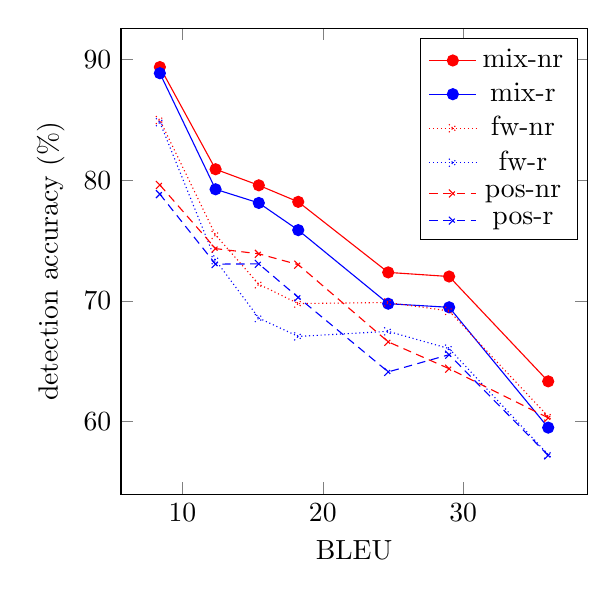
\begin{tikzpicture}
	\begin{axis}[width=7.5cm,height=7.5cm,
		xlabel= BLEU,ylabel=detection accuracy (\%)%,nodes near coords={(\coordindex)},
			]		

	\addplot[color=red,mark=*,style=solid] coordinates { %svm
		(36.06,	63.34)	%Google Translate
		(29,	72.02)		%Moses
		(24.66,	72.36)	%Systran
		(18.25,	78.20)	%Promt
		(15.44,	79.57)	%Linguatec
		(12.36,	80.90)	%Skycode
		(8.39 ,	89.36)	%Trident
	};
	\addlegendentry{mix-nr}
	
	\addplot[color=blue,mark=*,style=solid] coordinates { %svm
		(36.06,	59.51)	%Google Translate
		(29,	69.47)	%Moses
		(24.66,	69.77)	%Systran
		(18.25,	75.86)	%Promt
		(15.44,	78.11)	%Linguatec
		(12.36,	79.24)	%Skycode
		( 8.39,	88.85)	%Trident
	};
	\addlegendentry{mix-r}
	
	\addplot[color=red,mark=x,style=densely dotted] coordinates {%BLEU score vs. detection accuracy - function words - SVM - MT vs. Non-Reference
		(36.06,	60.43)	%Google Translate
		(29,	69.17)		%Moses
		(24.66,	69.87)	%Systran
		(18.25,	69.78)	%Promt
		(15.44,	71.38)	%Linguatec
		(12.36,	75.46)	%Skycode
		( 8.39,	84.97)	%Trident
	};
%	\addlegendentry{function-SVM-nonref}
	\addlegendentry{fw-nr}
	
	\addplot[color=blue,mark=x,style=densely dotted] coordinates {%BLEU score vs. detection accuracy - function words - SVM - MT vs. Reference
		(36.06,	57.27)	%Google Translate
		(29,	66.05)		%Moses
		(24.66,	67.48)	%Systran
		(18.25,	67.06)	%Promt
		(15.44,	68.58)	%Linguatec
		(12.36,	73.37)	%Skycode
		( 8.39,	84.79)	%Trident
	};
	%\addlegendentry{function-SVM-ref}
	\addlegendentry{fw-r}
	
	\addplot[color=red,mark=x,style=densely dashed] coordinates {%BLEU score vs. detection accuracy - POS unigrams - SVM - MT vs. Non-Reference
		(36.06,	60.32)	%Google Translate
		(29,	64.39)		%Moses
		(24.66,	66.61)	%Systran
		(18.25,	73)	%Promt
		(15.44,	73.90)		%Linguatec
		(12.36,	74.33)	%Skycode
		( 8.39,	79.60)	%Trident
	};
	%\addlegendentry{pos-SVM-nonref}
	\addlegendentry{pos-nr}
	
	\addplot[color=blue,mark=x,style=densely dashed] coordinates {%BLEU score vs. detection accuracy - POS unigrams - SVM - MT vs. Reference 
		(36.06,	57.21)	%Google Translate
		(29,	65.55)		%Moses
		(24.66,	64.1225)	%Systran
		(18.25,	70.29)	%Promt
		(15.44,	73.065)	%Linguatec
		(12.36,	73.0475)	%Skycode
		( 8.39,	78.84)	%Trident
	};
	\addlegendentry{pos-r}
	
	\end{axis}%
\end{tikzpicture}%
\caption{Correlation between detection accuracy and BLEU score on commercial MT systems, using POS, function words and mixed features against reference and non-reference sentences.}
\label{fig:detection-BLEU-correlation}
\end{figure}

As can be seen, best detection results are obtained using the full combined feature set. It can also be seen that, as might be expected, it is easier to distinguish machine-translated sentences from a non-reference set than from the reference set. In Figure \ref{fig:detection-BLEU-correlation}, we show the relationship of the observed detection accuracy for each system with the BLEU score of that system. As is evident, regardless of the feature set or non-MT sentences used, the correlation between detection accuracy and BLEU score is very high, as we can also see from the $R^2$ values in Table \ref{table:detection-detail}. 

\begin{table*}[ht]
\centering  % used for centering table
\begin{tabular}{c c c c c c c c c c c} % centered columns (4 columns)
\hline\hline                        %inserts double horizontal lines
Features & Data & Google & Moses & Systran & ProMT & Linguatec & Skycode & Trident & $R^2$ \\ [0.5ex] % inserts table 
%heading
\hline % inserts single horizontal line
mixed & MT/non-ref & \textbf{63.34} & \textbf{72.02} & \textbf{72.36} & \textbf{78.2} & \textbf{79.57} & \textbf{80.9} & \textbf{89.36} & 0.946 \\
mixed & MT/ref & 59.51 & 69.47 & 69.77 & 75.86 & 78.11 & 79.24 & 88.85 & 0.944 \\
func. w. & MT/non-ref & 60.43 & 69.17 & 69.87 & 69.78 & 71.38 & 75.46 & 84.97 & 0.798 \\
func. w. & MT/ref & 57.27 & 66.05 & 67.48 & 67.06 & 68.58 & 73.37 & 84.79 & 0.779 \\
POS & MT/non-ref & 60.32 & 64.39 & 66.61 & 73 & 73.9 & 74.33 & 79.6 & \textbf{0.978} \\
POS & MT/ref & 57.21 & 65.55 & 64.12 & 70.29 & 73.06 & 73.04 & 78.84 & 0.948 \\
%CFG & MT/non-ref & \\
%non-ter & MT/ref & \\

%POS-NB-Nonref & 57.85 & 61.04 & 62.51 & 71.11 & 68.3 & 68.61 & 74.07 \\ [1ex]      % [1ex] adds vertical space
\hline %inserts single line
\end{tabular}
\caption{Classifier performance, including the $R^2$ coefficient describing the correlation with BLEU. } % title of Table
\label{table:detection-detail} % is used to refer this table in the text
\end{table*}


% A comparison of outputs from several MT systems
\begin{table*}[t]
  \centering
  \begin{tabular}{*{2}{c}}
    \hline
    MT Engine & Example \\
    \hline
    Google Translate & "\textbf{These} days, \textbf{all} \textbf{but} \textbf{one} \textbf{were} subject \textbf{to} \textbf{a} vote, \\
    & \textbf{and} \textbf{all} \textbf{had} \textbf{a} direct link \textbf{to} \textbf{the} post September 11th." \\
	\hline
    Moses & "\textbf{these} days , \textbf{except} \textbf{one} \textbf{were} \textbf{the} subject \textbf{of} \textbf{a} vote , \\
	& \textbf{and} \textbf{all} \textbf{had} \textbf{a} direct link \textbf{with} \textbf{the} \textbf{after} 11 September ." \\
	\hline
    Systran & "\textbf{From} \textbf{these} days, \textbf{all} \textbf{except} \textbf{one} \textbf{were} \textbf{the} object \textbf{of} \textbf{a} vote, \\
 	& \textbf{and} \textbf{all} \textbf{were} connected \textbf{a} direct link \textbf{with} \textbf{after} September 11th." \\
    \hline
	Linguatec & "\textbf{Of} \textbf{these} days, \textbf{all} \textbf{except} \textbf{one} \textbf{were} making \textbf{the} object \textbf{of} \textbf{a} vote \\
	& \textbf{and} \textbf{all} \textbf{had} \textbf{a} straightforward tie \textbf{with} \textbf{after} September 11." \\
    \hline
	ProMT & "\textbf{These} days, \textbf{very} safe \textbf{one} \textbf{all} made object \textbf{a} vote, \\ 
	& \textbf{and} \textbf{had} \textbf{a} direct link \textbf{with} \textbf{after} September 11th." \\
    \hline
	Trident & "\textbf{From} \textbf{these} \textbf{all} days, \textbf{except} \textbf{one} operated object voting, \\
	& \textbf{and} \textbf{all} \textbf{had} \textbf{a} direct rope \textbf{with} \textbf{after} 11 septembre." \\
    \hline
	Skycode & "\textbf{In} \textbf{these} days, \textbf{all} safe \textbf{one} made \textbf{the} object \textbf{in} \textbf{a} vote \\
	& \textbf{and} \textbf{all} \textbf{had} \textbf{a} direct connection \textbf{with} \textbf{him} \textbf{after} 11 \textbf{of} September." \\
    \hline
	%Google Translate & "After Sept. 11, its economic forecasts do not reflect reality." \\
	%%\hline
	%    Moses & "after 11 September , its economic forecasts do not reflect reality ." \\
	%%\hline
	%    Systran & "After September 11th, its economic forecasts do not reflect reality." \\
	%    %\hline
	%Linguatec & "After September 11, its economical estimates do not reflect the reality." \\
	%    %\hline
	%ProMT & "After September 11th, its economic predictions do not reflect reality." \\
	%    %\hline
	%Trident & "After 11 septembre, his economic foresights do not reflect reality ." \\
	%    %\hline
	%Skycode & "After the 11 September, its economic anticipations do not reflect the world." \\
  \end{tabular}
\caption{Outputs from several MT systems for the same source sentence (function words marked in bold)}
\end{table*}

\subsection{In-House SMT Systems}
% List of machine translation systems
%\vspace{-3 mm}
\begin{table}[ht]
\centering  % used for centering table
\begin{tabular}{c c c c} % centered columns (4 columns)
\hline\hline                        %inserts double horizontal lines
 & Parallel & Monolingual & BLEU \\ [0.5ex] % inserts table 
%heading
\hline                  % inserts single horizontal line   SS SW WS WW 
SMT-1 & 2000k & 2000k & 28.54 \\ %BLEU = 28.54, 60.9/34.3/21.8/14.5 (BP=1.000, ratio=1.069, hyp_len=1073968, ref_len=1004791) 
SMT-2 & 1000k & 1000k & 27.76 \\ %BLEU = 27.76, 60.6/33.5/21.1/13.9 (BP=1.000, ratio=1.066, hyp_len=1070949, ref_len=1004791)
SMT-3 & 500k & 500k & 29.18 \\ %BLEU = 29.18, 62.1/34.9/22.3/15.0 (BP=1.000, ratio=1.030, hyp_len=1034561, ref_len=1004791)
SMT-4 & 100k & 100k & 23.83 \\ 
SMT-5 & 50k & 50k & 24.34 \\ %BLEU = 24.34, 57.8/29.8/17.9/11.4 (BP=1.000, ratio=1.060, hyp_len=1065330, ref_len=1004791)
SMT-6 & 25k & 25k & 22.46 \\ %BLEU = 22.46, 56.0/27.6/16.2/10.2 (BP=1.000, ratio=1.070, hyp_len=1075324, ref_len=1004791)
SMT-7 & 10k & 10k & 20.72 \\ %BLEU = 20.72, 54.1/25.6/14.6/9.1 (BP=1.000, ratio=1.074, hyp_len=1078749, ref_len=1004791)
[1ex] %inserting body of the table 

\hline %inserts single line
\end{tabular}
\caption{Details for Moses based SMT systems} % title of Table
\label{table:moses} % is used to refer this table in the text
\end{table}

In the second experiment set, we test our detection method on SMT systems we created, in which we have control over the training data and the expected overall relative translation quality. In order to do so, we use the Moses statistical machine translation toolkit \cite{conf/acl/KoehnHBCFBCSMZDBCH07}. To train the systems, we take a portion of the Europarl corpus \cite{koehn2005epc}, creating 7 different SMT systems, each using a different amount of training data, for both the translation model and language model. We do this in order to create different quality translation systems, details of which are described in Table \ref{table:moses}. For purposes of classification, we use the same content independent features as in the previous experiment, based on function words and POS tags, again with SMO-based SVM as the classifier. For data, we use 20,000 random, non reference sentences from the Hansard corpus, against 20,000 sentences from one MT system per experiment, again resulting in 40,000 sentence instances per experiment. The relationship between the detection results for each MT system and the BLEU score for that system, resulting in $R^2 = 0.774$, is shown in Figure \ref{fig:detection-BLEU-correlation-moses}.

\begin{figure}
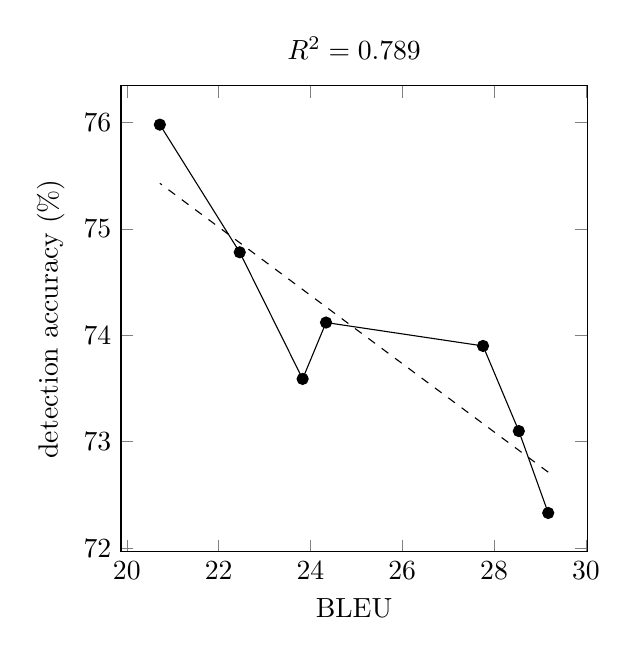
\begin{tikzpicture}
	\begin{axis}[title={$R^2 = 0.789$},width=7.5cm,height=7.5cm,
		xlabel= BLEU,ylabel=detection accuracy (\%)%,nodes near coords={(\coordindex)},
			]
	\addplot[color=black,mark=*] coordinates {%BLEU score vs. detection accuracy - POS unigrams - SVM - MT vs. Reference 
		(29.18,72.33)	%500k
		(28.54,73.10)	%2000k
		(27.76,73.90)	%1000k
		(24.34,74.12)	%50k
		(23.83,73.59)	%100k
		(22.46,74.78)	%25k
		(20.72,75.98)	%10k
	};
	%\addlegendentry{pos-r}

	\addplot[color=black,mark=none,style=dashed] table[
			y={create col/linear regression={y=Y}}] % compute a linear regression from the input table
		{
			% ordered pairs:
			% 19 out of 21
			% 0.904761904762
			% R^2 = 0.789
			X Y
			29.18 72.33
			28.54 73.10
			27.76 73.90
			24.34 74.12
			23.83 73.59
			22.46 74.78
			20.72 75.98
		};
		\xdef\slope{\pgfplotstableregressiona} %<-- might be handy occasionally

	\end{axis}%
\end{tikzpicture}%
\caption{Correlation between detection accuracy and BLEU score on in-house Moses-based SMT systems against non-reference sentences using content independent features.}
\label{fig:detection-BLEU-correlation-moses}
\end{figure}

\begin{figure}
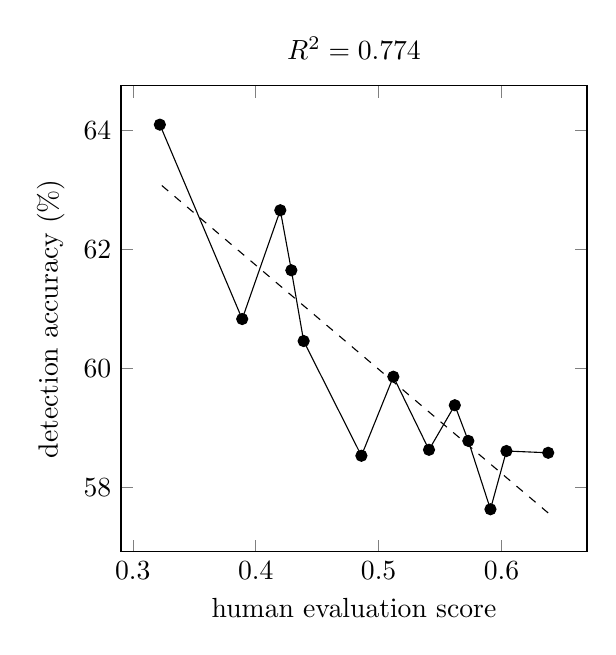
\begin{tikzpicture}
	\begin{axis}[title={$R^2 = 0.774$}, width=7.5cm,height=7.5cm,
		xlabel= human evaluation score,ylabel=detection accuracy (\%)%,nodes near coords={(\coordindex)},
			]
	\addplot[color=black,mark=*] coordinates {
		(0.638,58.58)	%uedin-heafield
		(0.604,58.61)	%uedin
		(0.591,57.63)	%online-b
		(0.573,58.78)	%limsi-soul
		(0.562,59.38)	%kit
		(0.541,58.63)	%online-a
		(0.512,59.86)	%mes-simplified
		(0.486,58.53)	%dcu
		(0.439,60.46)	%rwth
		(0.429,61.65)	%cmu-t2t
		(0.420,62.66)	%cu-zeman
		(0.389,60.83)	%JHU
		(0.322,64.10)	%SHEF
	};
	
	\addplot[color=black,mark=none,style=dashed] table[
			y={create col/linear regression={y=Y}}] % compute a linear regression from the input table
		{
			% correctly ordered pairs
			% 66 out of 78
			% 0.846153846154
			% r^2 = 0.7744
			% without JHU:
			% r^2 = 0.8054 
			% 56 out of 66 are ordered pair
			% 0.848484848485
			X Y
			0.638 58.58
			0.604 58.61
			0.591 57.63
			0.573 58.78
			0.562 59.38
			0.541 58.63
			0.512 59.86
			0.486 58.53
			0.439 60.46
			0.429 61.65
			0.420 62.66
			0.389 60.83
			0.322 64.10
		};
		\xdef\slope{\pgfplotstableregressiona} %<-- might be handy occasionally
		%\addlegendentry{$y(x)$}
		%\addlegendentry{% 
		%	$\pgfmathprintnumber{\pgfplotstableregressiona} \cdot x  
		%	\pgfmathprintnumber[print sign]{\pgfplotstableregressionb}$}

	\end{axis}%
\end{tikzpicture}%
\caption{Correlation between detection accuracy and human evaluation scores on systems from WMT13' against reference sentences. \newline}%workshop using pos+function words vs. reference 
\label{fig:human-detection-correlation-reference}
\end{figure}

\begin{figure}
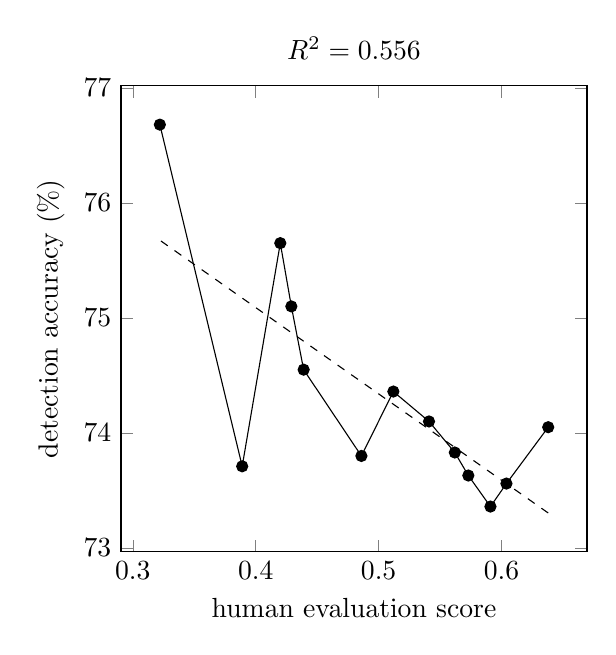
\begin{tikzpicture}
	\begin{axis}[title={$R^2 = 0.556$}, width=7.5cm,height=7.5cm,
		xlabel= human evaluation score,ylabel=detection accuracy (\%)%,nodes near coords={(\coordindex)},
			]
\addplot[color=black,mark=*] coordinates {
 	(0.638,74.05)	%uedin-heafield
 	(0.604,73.56)	%uedin
 	(0.591,73.36)	%online-b
 	(0.573,73.63)	%limsi-soul
 	(0.562,73.83)	%kit
 	(0.541,74.10)	%online-a
 	(0.512,74.36)	%mes-simplified
 	(0.486,73.80)	%dcu
 	(0.439,74.55)	%rwth
 	(0.429,75.10)	%cmu-t2t
 	(0.420,75.65)	%cu-zeman
 	(0.389,73.71)	%JHU
 	(0.322,76.68)	%SHEF
 };
\addplot[color=black,mark=none,style=dashed] table[
		y={create col/linear regression={y=Y}}] % compute a linear regression from the input table
	{
		% correctly ordered pairs
		% 61 out of 78
		% 0.782051282051
		% r^2 = 0.5563
		%without JHU:
		% r^2 = 0.7893 
		%57 out of 66 are ordered pairs
		%0.863636363636
		X Y
		0.638 74.05
		0.604 73.56
		0.591 73.36
		0.573 73.63
		0.562 73.83
		0.541 74.10
		0.512 74.36
		0.486 73.80
		0.439 74.55
		0.429 75.10
		0.420 75.65
		0.389 73.71
		0.322 76.68
	};
	\xdef\slope{\pgfplotstableregressiona} %<-- might be handy occasionally
	%\addlegendentry{$y(x)$}
	%\addlegendentry{% 
	%	$\pgfmathprintnumber{\pgfplotstableregressiona} \cdot x  
	%	\pgfmathprintnumber[print sign]{\pgfplotstableregressionb}$}

 %\addlegendentry{SMO-in}

	\end{axis}%
\end{tikzpicture}%
\caption{Correlation between detection accuracy and human evaluation scores on systems from WMT 13' against non-reference sentences. %from newstest 2010-2011 
}%workshop using pos+function words vs. reference
\label{fig:human-detection-correlation-non-reference}
\end{figure}

\begin{figure}
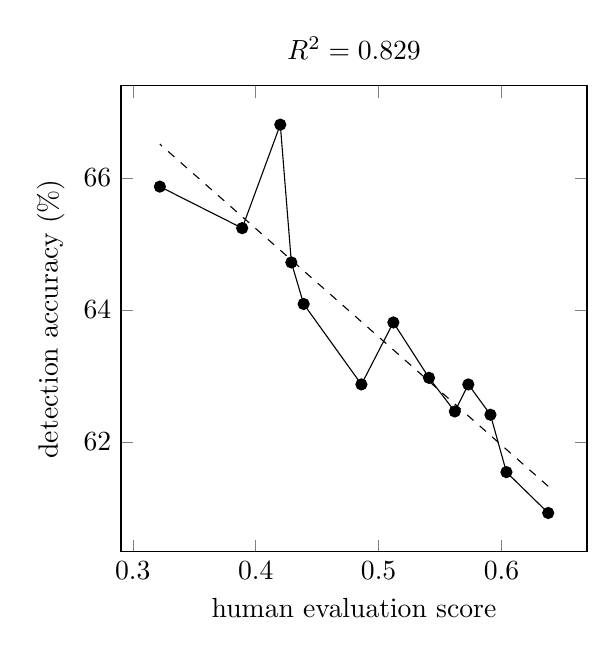
\begin{tikzpicture}
	\begin{axis}[title={$R^2 = 0.829$}, width=7.5cm,height=7.5cm,
		xlabel= human evaluation score,ylabel=detection accuracy (\%)%,nodes near coords={(\coordindex)},
			]
\addplot[color=black,mark=*] coordinates {
 	(0.638,60.92)	%uedin-heafield
 	(0.604,61.54)	%uedin
 	(0.591,62.41)	%online-b
 	(0.573,62.87)	%limsi-soul
 	(0.562,62.46)	%kit
 	(0.541,62.97)	%online-a
 	(0.512,63.81)	%mes-simplified
 	(0.486,62.87)	%dcu
 	(0.439,64.09)	%rwth
 	(0.429,64.72)	%cmu-t2t
 	(0.420,66.81)	%cu-zeman
 	(0.389,65.24)	%JHU
 	(0.322,65.87)	%SHEF
 };
\addplot[color=black,mark=none,style=dashed] table[
		y={create col/linear regression={y=Y}}] % compute a linear regression from the input table
	{
		% correctly ordered pairs
		%72 out of 78
		%0.923076923077
		% r^2 = 0.8291
		X Y
		0.638 60.92
		0.604 61.54
		0.591 62.41
		0.573 62.87
		0.562 62.46
		0.541 62.97
		0.512 63.81
		0.486 62.87
		0.439 64.09
		0.429 64.72
		0.420 66.81
		0.389 65.24
		0.322 65.87
	};
	\xdef\slope{\pgfplotstableregressiona} %<-- might be handy occasionally
	%\addlegendentry{$y(x)$}
	%\addlegendentry{% 
	%	$\pgfmathprintnumber{\pgfplotstableregressiona} \cdot x  
	%	\pgfmathprintnumber[print sign]{\pgfplotstableregressionb}$}

 %\addlegendentry{SMO-in}

	\end{axis}%
\end{tikzpicture}%
\caption{Correlation between detection accuracy and human evaluation scores on systems from WMT 13' against non-reference sentences, using the syntactic CFG features described in section 4.2 %from newstest 2010-2011 
}%workshop using pos+function words vs. reference
\label{fig:human-detection-correlation-non-reference-CFG}
\end{figure}

\section{Machine Translation Evaluation}

\subsection{Human Evaluation Experiments}
As can be seen in the above experiments, there is a strong correlation between the BLEU score and the MT detection accuracy of our method. In fact, results are linearly and negatively correlated with BLEU, as can be seen both on commercial systems and our in-house SMT systems. We also wish to consider the relationship between detection accuracy and a human quality estimation score. To do this, we use the French-English data from the 8th Workshop on Statistical Machine Translation - WMT13' \cite{bojar-EtAl:2013:WMT}, containing outputs from 13 different MT systems and their human evaluations. We conduct the same classification experiment as above, with features based on function words and POS tags, and SMO-based SVM as the classifier. We first use 3000 reference sentences from the WMT13' English reference translations, against the matching 3000 output sentences from one MT system at a time, resulting in 6000 sentence instances per experiment. As can be seen in Figure \ref{fig:human-detection-correlation-reference}, the detection accuracy is strongly correlated with the evaluations scores, yielding $R^2 = 0.774$. To provide another measure of correlation, we compared every pair of data points in the experiment to get the proportion of pairs ordered identically by the human evaluators and our method, with a result of $0.846$ (66  of 78). In the second experiment, we use 3000 random, non reference sentences from the newstest 2011-2012 corpora published in WMT12' \cite{callisonburch-EtAl:2012:WMT} against 3000 output sentences from one MT system at a time, again resulting in 6000 sentence instances per experiment. While applying the same classification method as with the reference sentences, the detection accuracy rises, while the correlation with the translation quality yields $R^2 = 0.556$, as can be seen in Figure \ref{fig:human-detection-correlation-non-reference}. Here, the proportion of identically ordered pairs is $0.782$ (61 of 78). 

\subsection{Syntactic Features}
We note that the second leftmost point in Figures \ref{fig:human-detection-correlation-reference}, \ref{fig:human-detection-correlation-non-reference} is an outlier: that is, our method has a hard time detecting sentences produced by this system although it is not highly rated by human evaluators. This point represents the Joshua \cite{citeulike:12539454} SMT system. This system is syntax-based, which apparently confound our POS and FW-based classifier, despite it's low human evaluation score. We hypothesize that the use of syntax-based features might improve results. To verify this intuition, we create parse trees using the Berkeley parser \cite{Petrov2007} and extract the one-level CFG rules as features. Again, we represent each sentence as a boolean vector, in which each entry represents the presence or absence of the CFG rule in the parse-tree of the sentence. %, denoted in: $f_{CFG}(s) = (z_1,...,z_m)\in\lbrace0,1\rbrace^m$, given there are $m$ CFG rule types in the vocabulary. 
Using these features alone, without the FW and POS tag based features presented above, we obtain an $R^2 = 0.829$ with a proportion of identically ordered pairs at $0.923$ (72 of 78), as shown in Figure \ref{fig:human-detection-correlation-non-reference-CFG}.
%We can see in the above experiments that the correlation between the detection accuracy and the translation quality is varied among the different experiment setups. For example, in the first two experiment sets, the $R^2$ values were very close when using either reference or non-reference sentences (as can be seen in Table \ref{table:detection-detail}), while there is a greater difference between those values in the 3rd experiment set, decreasing from $R^2 = 0.774$ with reference sentences to $R^2 = 0.556$ with non-reference sentences as seen in Figures \ref{fig:human-detection-correlation-reference} and \ref{fig:human-detection-correlation-non-reference}. We explain this mainly as a result of the amount of instances involved in the experiment, as in the first experiment sets we had 40,000 sentences per experiment, and in the last set we had 6000 sentences involved in each experiment. %As our method measures the detection accuracy over the sentences, it is more sensitive to errors when using less data. Having that said, we can still see consistent correlation even in the latter experiment set, when observing the proportion of correctly correlated pairs, which is less affected by singular errors, decreasing from $0.846$ to $0.782$, while handling errors as we can see with the 2nd data point, in Figures \ref{fig:human-detection-correlation-reference} and \ref{fig:human-detection-correlation-non-reference}.


\section{Discussion and Future Work}

We have shown that it is possible to detect machine translation from monolingual corpora containing both machine translated text and human generated text, at sentence level. There is a strong correlation between the detection accuracy that can be obtained and the BLEU score or the human evaluation score of the machine translation itself. This correlation holds whether or not a reference set is used. This suggests that our method might be used as an unsupervised quality estimation method when no reference sentences are available, such as for resource-poor source languages. %This implies that using features such as the presence or absence of function words, parts of speech or syntactic relations can predict the quality of a given translation system. 
Further work might include applying our methods to other language pairs and domains, acquiring word-level quality estimation or integrating our method in a machine translation system. Furthermore, additional features and feature selection techniques can be applied, both for improving detection accuracy and for strengthening the correlation with human quality estimation.

\section*{Acknowledgments}

We would like to thank Noam Ordan and Shuly Wintner for their help and feedback on the early stages of this work. This research was funded in part by the Intel Collaborative Research Institute for Computational Intelligence.

\vspace{10 mm}
%\vspace{10mm}
% include your own bib file like this:
\bibliographystyle{acl}
\bibliography{bibliography}

\end{document}
